\documentclass[conference]{IEEEtran}
\usepackage{amsmath,amssymb,amsfonts}
\usepackage{algorithmic}
\usepackage{graphicx}
\usepackage{textcomp}
\usepackage{xcolour}
\usepackage[backend=biber, sorting=none]{biblatex}
\usepackage{lipsum}
\usepackage{url}
\usepackage{subcaption}
\usepackage[colorlinks=true, urlcolor=blue, pdfborder={0 0 0}]{hyperref}
\addbibresource{bibliography.bib}
\def\BibTeX{{\rm B\kern-.05em{\sc i\kern-.025em b}\kern-.08em
    T\kern-.1667em\lower.7ex\hbox{E}\kern-.125emX}}

\begin{document}


	\title{Proposition of a New Experiment to Better Understand the Relation Between Typicality and Prototypes}


	\author{\IEEEauthorblockN{Samuel Kostadinov}
	\textit{University of Trento}\\
	Trento, Italy \\
	samuel.kostadinov@studenti.unitn.it}


	\maketitle


	\begin{abstract}
		
		The typicality is a topic that still needs exploration. In this paper, the proposed experiment makes use of feature extraction to build a prototype and a siamese network to find a possible correlation 
		between the typicality of a concepts and the similarity between a given image and the built prototype. 
		
	\end{abstract}

	\begin{IEEEkeywords}
		Typicality, Prototypes, CNNs, Siamese Network
	\end{IEEEkeywords}


	\section{Introduction}
		
		\noindent The typicality of a concept is a topic that needs a lot of exploration, since it's difficult to evaluate precisely the typicality of an object 
		and also because the people's brains are always a little different from each other. The experiment I would like to propose, has the objective of 
		making us understand better the bond between the perceived typicality of an object that belongs to a category and the prototype of that category.
		This can help the scientists to better understand how knowledge is organized in the brain. This experiment consists in different phases, such as
		data collection, feature extraction, prototype construction and similarity judgment.


	\section{Background}

		\subsection{Feature extraction}

			\noindent Feature extraction is a topic widely studied. 
			This topic has numerous different applications. 
			One of its goals is to reduce the amount of computational power needed for image processing. 
			There are various techniques to extract meaningful features from images. 
			Some of them are very common and very easy to implement. 
			These are, for example, edge extraction or shape analysis. 
			Other possibilities, more advanced, involve neural networks.\\

				\subsubsection{Classic feature extraction techniques}
					
					One of the first feature extraction methods implemented in image processing is edge detection.				
					In 2019, a paper by Owotogbe presented a review of edge detection techniques. 
					These are usually divided into two groups, gradient-based and Gaussian-based. 
					Some examples are the Sobel operator and the Canny edge detector. 
					Each of the methods has pros and cons. 
					It's the user's job to find the most appropriate for its goal~\cite{owotogbe2019edge}.\\
					
					\begin{figure*}[!ht]
						\centering
						\begin{subfigure}[!ht]{0.48\linewidth}
							\centerline{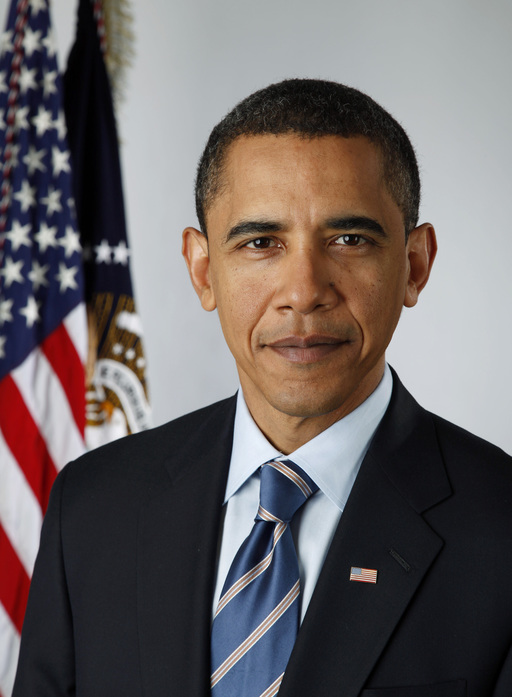
\includegraphics[width=0.9\linewidth]{imgs/obama.jpg}}
							\label{fig:1a}
						\end{subfigure}
						\begin{subfigure}[!ht]{0.48\linewidth}
							\centerline{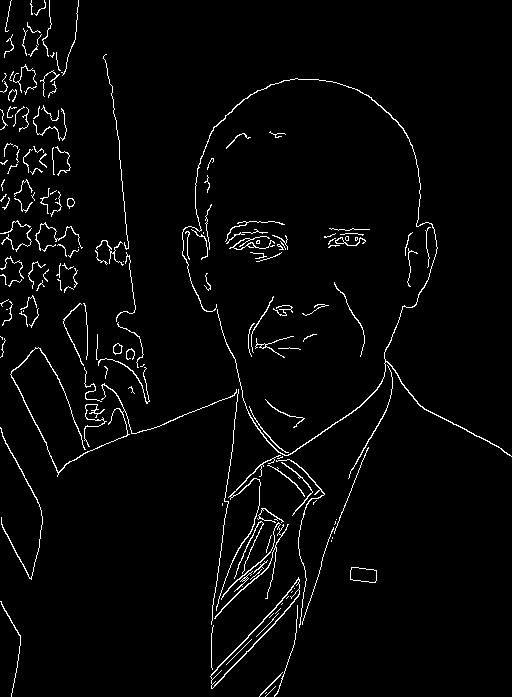
\includegraphics[width=0.9\linewidth]{imgs/obama_edges.jpg}}
							\label{fig:1a}
						\end{subfigure}
						\caption{Example of edge detection}
						\label{fig:1}
					\end{figure*}
					
					\noindent After edge detection, other techniques began to spread for feature extraction. 
					In a paper by Kumar and Kumar Bhatia written in 2014 \cite{kumar2014detailed}, 
					there are some examples of techniques used to extract features. 
					In the first one, the authors present different types of features and then some techniques to extract them. 
					These are:

					\begin{itemize}
					
						\item \textbf{Diagonal based feature extraction techniques}:
						
							In this procedure, the image is divided into zones formed by small squares of pixels. 
							In the paper's case, there would be 19 diagonal lines. 
							The value of each pixel in these diagonals is summed to obtain a single sub feature. 
							Then we can extract a feature by averaging the sub features. 
							With this method, we can extract a feature for every zone. 
							Then by averaging the column-wise and row-wise features we can increase their number. 
							
						
						\item \textbf{Fourier descriptors}:
						
							The Fourier transform is commonly used for shape analysis. 
							The Fourier transformed coefficient form the Fourier descriptors. 
							These descriptors represent the shape in a frequency domain, with the low frequencies symbolizing the general shape and the high frequencies symbolizing details of the shape. 
							Since the transformation usually generates many parameters, only a subset is considered.
						
						
						\item \textbf{Principal Component Analysis (PCA)}:
						
							This procedure is a mathematical way to convert a set of observations into a set of values of uncorrelated variables. 
							These variables are defined so that the first one has the highest variance, and the components are all orthogonal (independent) from each other. 
							
						\item \textbf{Independent component analysis (ICA)}:
						
							ICA is a statistical technique. 
							It aims to use non-Gaussian random variables to represent multidimensional vectors. 
							The random variables should be as independent as possible. 
						
						\item \textbf{Gabor filter}:
						
							A Gabor is a sinusoid multiplied by a Gaussian, and its response is a convolution operation. 
							This type of filter performs well in both spatial and frequency domains. 
						
						\item \textbf{Chain Code Histogram of Character Contour}:
						
							This method is based on a contour following technique. 
							The contour following uses a chain coding standard proposed by Freeman, that assigns a value to every pixel to identify the next pixel in the border.

						\item \textbf{Finding Intersection/Junction in character}:
						
							Using the same standard proposed by Freeman used in Chain Code Histogram, there is the possibility to count intersections (or junctions) and open ends in a figure.					
							
						\item \textbf{Transition feature}:
						
							This method is based on the transition from background to foreground. 
							There are different techniques that can work both on gray level images or in 4-connected or 8-connected images.
						
					\end{itemize}
				
				
				\noindent These were not the only techniques presented in the paper, but since some were more problem-specific (about handwritten character recognition)
				were excluded from the list. These excluded techniques can still be used, but may have worse results or may require some adaptation. 
				The techniques were: Fractal theory techniques, Shadow features of character, Sector approach for feature extraction, 
				Extraction of distance and angle features, Extraction of occupancy and end-point features, and Zernike moments.\\
				In another paper, written in 2013 by Tian \cite{ping2013review}, there are some other techniques cited that may result useful:
				
				\begin{itemize}
				
					\item \textbf{colour features}:
						
						colour is one of the most important features humans can perceive. 
						The features we can extract depend on the colour space, but once it's defined there are some possibilities. 
						A few examples are colour histograms, colour moments and colour coherence vectors. 
						One of the simple and meaningful, according to the authors, is colour moments. 
						The most common colour moments are the mean, the standard deviation and the skewness. 
						
					\item \textbf{Texture features}:
					
						Another very important feature of images is texture. 
						Features involving texture analysis can be extracted from groups of pixels. 
						One of the most common methods is a Gabor filter, which can be used by characterizing the central frequency and the orientation parameters.
				
				\end{itemize}
				
				\begin{figure}[!ht]
					\centerline{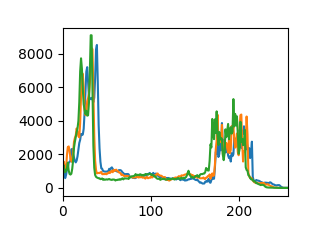
\includegraphics[width=\linewidth]{imgs/obama_histogram.png}}
					\caption{Example of color histogram}
					\label{fig:2}
				\end{figure}
				
				\subsubsection{Deformable shape analysis}
			
					A more sophisticated technique than the ones listed before is shape analysis. Deformable shape analysis, in particular, can be useful to extract features from an image.\\
					In 2005, Felzenszwalb wrote a paper that focuses on representation and detection of deformable shapes~\cite{felzenszwalb2005representation}. For the goal of the experiment proposed here, some deformable shape 
					detection techniques can be useful. \\
					The technique proposed strongly relies on the triangulated polygon representation. This type of representation lets approximate every 2D shape without holes using a representation based on triangles. 
					%The resulting approximation is as precise as the user decides, meaning that it's very flexible for the representation of shapes. 
					%In particular, in the paper the triangulation was done with a technique called constrained Delaunay triangulation (CDT), because of its tight relation with the medial axis transform. 
					The author also make use of the properties of chordal graphs and k-trees.\\
					The technique described in this paper falls under the category of deformable template matching. One of the components of the method is the energy function, a function that associates a cost with every 
					possible transformation. The objective is to find the transformation with the lowest possible cost. This component is very flexible, since depending on the formulation of the energy function the costs 
					can be tuned even for individual triangles. Moreover, it is also possible to integrate learning techniques to learn deformation parameters.
					Since the possible non-rigid transformations of a template are numerous, this kind of techniques usually requires an initialization near to the correct solution, 
					although this is not required for the algorithm presented in this paper. 
					For the implementation of the algorithm itself, a techniques called non-serial dynamic programming was the key factor. In fact, using the order of perfect elimination (property of the every triangulated 
					simple polygon), the algorithm computes the optimal position of every vertex with respect to the other vertices. Once the algorithm solves for the last vertex, it can 
					update all the others as in typical dynamic programming and obtain the optimal location for every vertex.\\
					The learning of the parameters can be seen as looking for the location with the highest. The matching problem is then fed to a statistical framework that computes the configuration minimizing the 
					energy cost, which corresponds to the best template match.
					
					\begin{figure}[!ht]
						\centerline{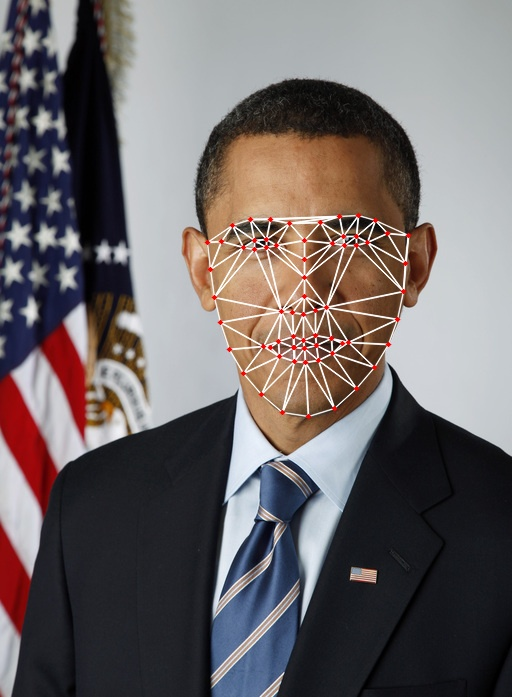
\includegraphics[height=0.4\textheight]{imgs/delaunay.jpg}}
						\caption{Example of delaunay triangulation, the type of triangulation at the base of Felzenszwalb's paper}
						\label{fig:3}
					\end{figure}
					
				\subsubsection{Machine learning based feature extraction techniques} \label{mlfe}
					
					After the classic techniques, machine learning began to be involved in feature extraction. In particular there are some papers that explain the results achieved with machine learning.\\
					In 2019, Halimi et al. wrote a paper about a feature extraction technique that they implemented using unsupervised deep learning~\cite{halimi2019unsupervised}. Although this paper examines the techniques for 
					3D shapes, it's very likely that it can be adapted to extract 2D features from images.\\
					The background of this experiments is formed of some concepts that are not immediate. One of the concepts used as background is the minimum distortion correspondence. The other are, for example, 
					descriptor learning, functional maps and deep functional maps. These concepts serve as a base for all the work done later. \\
					In particular, the authors focus on unsupervised deep functional maps. The authors state that the main contribution of their paper is that they introduce a technique with which they can 
					avoid annotating a lot of data before training a model. After reducing the number of vertices to a number between 5000 and 7000, the authors used a deep functional map network. The inputs are 
					fed to two residual neural networks, which compute a dense descriptor fields. These descriptors, are the inputs to the functional map layer. Lastly, as post processing, a point-wise map recovery was 
					applied and, after that, the shape was upscaled to the original resolution. 
					
					\noindent In 2019, there is another paper, written by Varshni et al. that proposes another method~\cite{varshni2019pneumonia}. This paper has the objective to classify images suing CNNs to understand if a patient 
					has pneumonia or not. After the preprocessing, in which the authors just resized the images, there is the feature extraction process. For this step, the authors used different pretrained models.
					In this paper's results it's reported that the best model architecture is DenseNet-169. This kind of neural network, called Dense Nets, overcomes the problem of gradient vanishing. The model used in 
					particular for the work of this paper had 4 dense blocks and 3 transition layers. Then there is a classification layer. 
					
					\noindent In 2019, Guamei et al. wrote a paper about hybrid feature extraction methods to classify brain tumours~\cite{gumaei2019hybrid}. The process described in the paper is divided into three points. The 
					first one is preprocessing, the second is feature extraction and the third is brain tumour classification. The first step is just to rescale the values to the range $[0,\ 1]$. The feature extractor 
					used is the GIST descriptor. The GIST is then combined with a Gabor filter and produces a total of $mxnx4x4$ GIST feature vectors. There is a variant of the GIST descriptor, the 
					PCA-NGIST is a PCA-based normalized GIST feature extraction method. The NGIST is a normalized version of the GIST descriptor, that uses the L2 norm to make the GIST invariant to illumination and shadowing. 
					After this step, the only thing left is the classification of the tumour, which was performed with a RELM classifier. 
					
					\begin{figure*}[!ht]
						\centerline{\includegraphics[width=\linewidth]{imgs/cnn_features.png}}
						\caption{Example of features extracted by a CNN}
						\label{fig:4}
					\end{figure*}	
					
					\noindent In Figure \ref{fig:4} there is an example of feature extracted by a Convolutional Neural Network. 
					
				\subsubsection{Hyperspectral images feature extraction}
					
					Although there exists techniques that can extract features from hyperspectral images, this kind of images are created to capture the entire spectrum. This fact means that these images can capture 
					more information then what the human eye can. techniques involve, in the majority of the cases, learning of some form, especially in form of neural networks, in particular convolutional recurrent 
					networks, as seen in a paper by Hu et al.~\cite{hu2020spatial} and in a paper by Rasti et al.~\cite{rasti2020feature}. For the reasons just said, it's probably more meaningful to use normal 
					images than these ones.
			
			\subsection{Networks}
			
				\noindent Neural Networks are a powerful instrument in the hands of computer scientists. There exists a lot of different types of artificial neural networks, each with its own peculiarities. In particular, for this 
				experiment the one needed will be, most likely, just convolutional neural networks and siamese neural networks. 
			
				\subsubsection{Convolutional Neural Network (CNN)}
				
					Convolutional neural networks are not an extremely recent type of neural network, especially if we consider that LeNet-5 was created in 1998. Scientists have dealt with CNNs for some years. Now, as of 2022, 
					CNNs are mostly used to deal with images.\\
					In 2017, Wu wrote a paper that had the purpose to serve as an introduction to CNNs~\cite{wu2017introduction}. These networks use mostly three kind of layers: Dense layers (which are fully connected layers), 
					convolution layers and pooling layers. In the following, there will be a short description of each kind of layer. 
					\begin{itemize}
						
						\item \textbf{Dense layer}:\\
							The dense layer is not peculiar of CNNs, in fact it's found in almost all types of neural networks. It consists of a set of neurons that are connected with every neuron of the previous 
							layer. Dense layers are usually used towards the end of the network.
						
						\item \textbf{Convolutional layer}:\\
							Convolutional layers just compute a convolution operation. This helps reducing the input size and extract meaningful features from the image taken as input. These layers are usually used 
							in the first layers of the neural network.
						
						\item \textbf{Pooling layers}:\\
							Pooling layers downsample the image to reducing the number of parameters needed. These layers are usually alternated with the convolution layers, so are used at the beginning of a neural network.
							
					\end{itemize}
					
					\noindent The applications of deep learning and CNNs are numerous. As shown previously, there are some CNNs used in image classification with the objective to identify diseases. The typical example is 
					the pneumonia detection. Another possibility is to use CNNs in segmentation or self driving cars, as stated in \cite{alzubaidi2021review} by Alzubaidi et al.
			
					\begin{figure}[!ht]
						\centerline{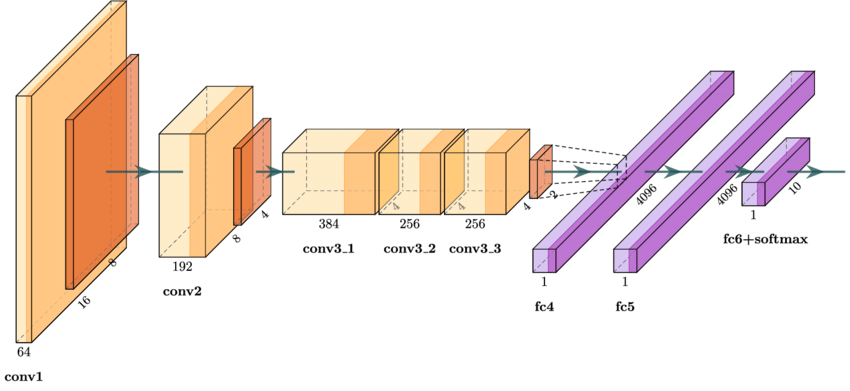
\includegraphics[width=\linewidth]{imgs/cnn_architecture.png}}
						\caption{Example of CNN architecture. In particular, this image represents AlexNet's architecture}
						\label{fig:5}
					\end{figure}
					
					\noindent In figure \ref{fig:5} there is an example of the architecture of a CNN, in particular AlexNet is the CNN chosen for this example. 
					
				\subsubsection{Siamese Neural Network}

					Siamese neural networks, also called twin networks, are a more recent advance in computer science. These neural networks have a different structure from convolutional neural networks. The 
					structure of siamese neural networks is peculiar. In fact, there are two identical networks, called embedding networks, that process different inputs and, after that, 
					merge in a single layer that measures the similarity between 
					the two outputs of the two networks. The siamese neural networks have a different application compared to CNNs, in fact twin networks are mainly used to measure similarity of two objects. 
					In the case of this paper, the siamese neural networks are used for image matching. This is not the first time that siamese networks are used for image matching, as proved by a paper written in 2016 by 
					Melekhov et al.~\cite{melekhov2016siamese}, but with a little difference in the objective of the matching. The objective of the paper was to learn a general similarity for image retrieval, while on the case of this 
					paper, the objective is to find a similarity measure with a prototype. 
					
					\begin{figure}[!ht]
						\centerline{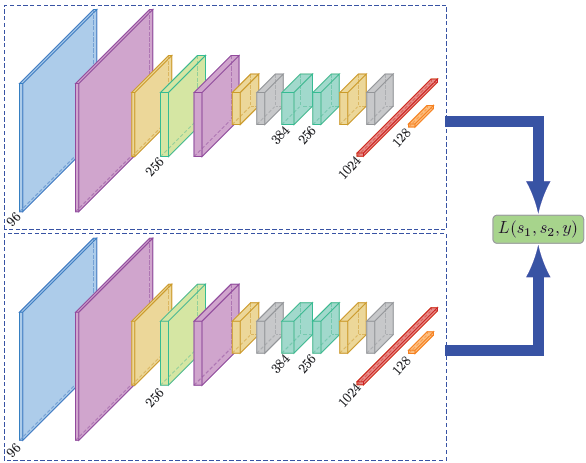
\includegraphics[width=\linewidth]{imgs/siamese_architecture.png}}
						\caption{Example of a Siamese Network architecture.}
						\label{fig:6}
					\end{figure}
					
					\noindent In Figure \ref{fig:6} there is an example of a Siamese Neural Network, in particular the two embeddings are convolutional neural networks. 
					
					% Training with triplets (?)
			
			\subsection{Similarity judgments}
				
				In the past there have been some works regarding image similarity, like for example the one presented by Appalaraju and Chaoji in 2017~\cite{appalaraju2017image}. In this work they explore the possibility to 
				find a similarity measure for image retrieval. To achieve this goal, they implemented a siamese neural network that uses two identical multi-scale CNNs that share weights. The ouput of the 
				network is binary, being $1$ the label to predict in case of negative examples and $0$ the label to predict in case of positive example. The loss function used in this work is a contrastive loss. This paper 
				then proceeds to explain a technique called Online Pair Mining Strategy (OPMS), inspired by curriculum learning, that helps reducing the training time. \\
				This is not the only work that uses neural networks to learn similarity, in fact there are also other application fields for similarity study. One of them is healthcare, as shown in a paper by Suo et al., written in 
				2017, that introduces a model used to make personalized prediction of diseases for patients, basing the prediction on a similarity related method, learned using CNNs~\cite{8217759}. In this paper, before 
				learning the actual similarity measure, the authors processed the input through a CNN and performed a step they call ``Time fusion''. This step let them incorporate the time information and 
				weight differently eventual symptoms based on their temporal distance from the onset of the disease. Only after this step the authors proceeded to learn a similarity metric, basing the learning 
				on CNNs.\\
				Another paper, written by Chopra et al. in 2005, used a method similar to the one written by Appalaraju. In this work, the authors used a siamese architecture to learn a similarity metric and applied it 
				in the field of face verification~\cite{chopra2005learning}.\\
				More interestingly, there are also other papers, in particular a paper by Attarian et al. written in 2020 uses $VGG16$. This paper's goal is to use this CNN to predict human similarity 
				judgments~\cite{attarian2020transforming}. Using $VGG16$, the authors were able to achieve good results, with over 90\% in validation accuracy.
				
	\section{Data Collection}

		\subsection{Image collection}
			
			\noindent Since the proposed experiment uses neural networks, there is the need to have a lot of data. In this particular case, there is the need to gather many images. There are some image dataset, intended for computer 
			vision~\footnote{\url{https://imerit.net/blog/22-free-image-datasets-for-computer-vision-all-pbm/}}, that could help. Some of the dataset reported there are famous, like ImageNet or Google's Open Images. The 
			best for this kind of work, though, is to have a dataset that bases every image on the same ``macro-category'', like for example a dataset made of images of birds.
		
		\subsection{Typicality values}
			
			\noindent In this experiment, typicality judgments play a crucial role. To gather enough data about the perceived typicality of images, a form is necessary. This survey should be structured in a way that presents an 
			image ad a time to the subject that is taking the survey and asks to rate the typicality of the object portrayed in the image, possibly in a given range. If that's the case, a range between $1$ and $10$ 
			could be the best decision since people are quite used to rate in this range. Once there are enough results, the various rates should be averaged so that there is a single measure that takes into 
			account every rate taken from the survey. The number of people that should participate in the experiment should be high enough to be a meaningful statistical group.

	\section{Feature Extraction\label{sec:fe}}

		\noindent While collecting the needed data with the survey, it's possible to begin the feature extraction procedure. There are various possibilities for this step, as shown in the Section dedicated to feature extraction background. 
		It could be interesting to test both classical and machine learning methods, to measure which one is the most efficient. Since feature extraction has already been described in the paper, this section will 
		present a discussion about the results of the presented methods' results. The main difference between the classical and the machine learning feature extraction techniques is human interpretability. 
		In fact, for classical feature extraction techniques, humans have no difficulty in interpreting the result of the process. For example, in edge extraction, humans have no difficulty in recognizing if the 
		edge extracted is correct or not seeing the original image. For example, in Figure \ref{fig:1} no one has any problem to recognize that the figure on the right is the one that draws the edges of the figure on the left, 
		while in Figure \ref{fig:4} there is no clear correlation between the feature and what it means in the image itself.
		Moreover, classical and machine learning features can give different weights to different features. 
		In fact, classical methods rely on features that humans consider important, on the basis of general experience about the world, but also based on the way our brain works. An empirical confirmation of this fact 
		can be that if a person asks to another person to describe, for example, a common kingfisher, the person that should describe the bird will, most likely, start describing the dimension, the shape, and only 
		later the colour. Machine learning techniques, on the other hand, could give a very high importance to the fact that the bird is mainly blue and red, if they have access to the colour information. Due to the fact that 
		the blue colour is not very present in nature, the blue and red couple of colours can be highly characteristic of the common kingfisher, even if humans give, unconsciously and innately, more importance to 
		shape-related features.	

	\section{Prototype construction}

		\noindent The construction of the prototype is one of the most delicate parts of the experiments. How this phase works depends heavily on what method was used for feature extraction. 
		
		\subsection{Classical feature extraction techniques}
		
			\noindent In case classical feature extraction techniques were used, the goal of this activity is to build an image that presents in itself a ``prototype'' of the object. For example, a prototype of a bird, could be 
			an imaginary bird with a shape that it's obtained with a weighted average of the shapes of all the birds in the image. For example, since a birds like sparrows and swallows are perceived as more 
			typical than ostriches and penguins the prototype should resemble more swallows and sparrows than ostriches and penguins. To do so, the key factor is performing numerous analyses on various 
			different subjects, until there are enough data to have a statistical value. 
			
			\begin{figure*}[!t]
				\centering
				\begin{subfigure}[!t]{0.48\linewidth}
					\centerline{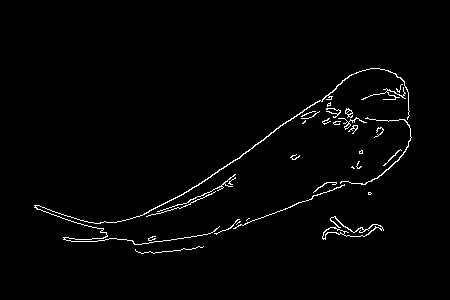
\includegraphics[width=0.9\linewidth]{imgs/swallow_edges.jpg}}
				\end{subfigure}
				\begin{subfigure}[!t]{0.48\linewidth}
					\centerline{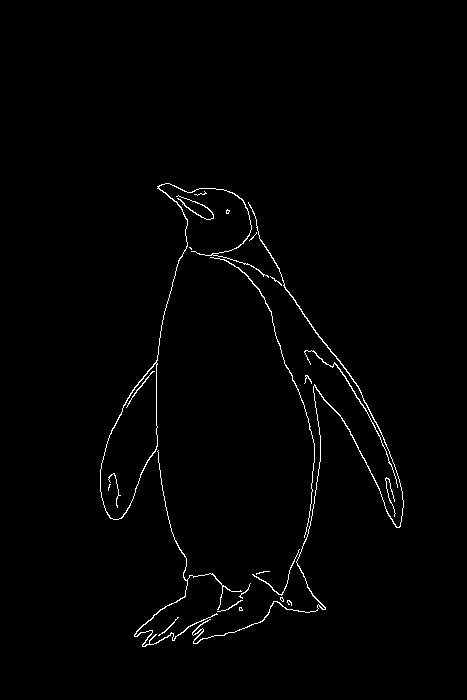
\includegraphics[height=0.4\textheight]{imgs/penguin_edges.jpg}}
				\end{subfigure}
				\caption{Edge extraction of swallow and penguin}
				\label{fig:7}
			\end{figure*}
		
		\noindent In Figure \ref{fig:7} there is an example of the edges of two different birds. Although both of the subjects of the original 
		subjects are birds, one is much more typical than the other one. In this case, the prototype should try to match more the swallow edge than the penguin edge. A way to do so could make use deformable 
		template matching. Matching a shape with a template could be useful to find a weighted average between the two shapes. In this way, the resulting shape takes into account both the original edges while 
		giving priority to the one more typical.
		This procedure should be applied for both shape features and colour features, so that all the features that can be extracted from the prototype image resemble the weighted average of all the feature from 
		the original images. 

		\subsection{Machine learning feature extraction techniques}
		
			\noindent In case machine learning feature extraction techniques were used, it's conceptually and practically easier to compute the average features. In fact, the features extracted by machine learning techniques are 
			in the form of arrays of numbers, so to compute the prototype of the image in this form it's enough to take the weighted average of the vectors.
		
		\subsection{Considerations about prototype construction}
		
			\noindent The prototype depends on the feature extraction technique that was used. As discussed in Section \ref{sec:fe}, the key difference is human interpretability. In fact, building a prototype using the 
			classical feature extraction methods, results in an image that can be seen and interpreted. Using a prototype generated with machine learning feature extraction techniques results in an array 
			of numerical values, that are not easily interpretable. As of 2022, there has been some research on the topic of interpretability and explainability of machine learning, like for example 
			a work by Carvalho written in 2019, %(\textbf{SOME CITATIONS}),
			but the field is still growing, also given the interest deriving from the AI-Act, the proposition of the european union in the field of artificial intelligence. In particular, there is a document of 
			the act~\footnote{\url{https://eur-lex.europa.eu/resource.html?uri=cellar:e0649735-a372-11eb-9585-01aa75ed71a1.0001.02/DOC_1&format=PDF}} that states that there will be some requirements in terms of 
			transparency and intepretability for machine learning systems that are considered high-risk AI. The growing interest produced some results, but still they're not enough to easily interpret machine learning 
			features.\\
			Most likely, in the future will be possible to look at the features extracted by a neural network and comprehend their meaning. When this will be possible, independently of the feature extraction techniques 
			used, the human interpretability will be possible, and with that in mind it would be probably more convenient to extract the features using neural networks. The reason behind this consideration is 
			that although the training of a neural network can be expensive in computational terms, the evaluation of an input on a trained network it's not very computationally demanding. On the other side, algorithms 
			like the triangulation always have the same demand, that is lower than the demand of training a neural network, but surely higher than the demand of evaluating a single input on a neural network. 
			Moreover, considering the possiblity to use transfer learning techniques, the training can become a fine-tuning or a domain adaptation, which means the computational load is lighter. Considering that 
			the fact that the training is a demanding task to be perfomed only once and that other algorithms may be less demanding but must be run multiple times, it's probably more convenient to train a neural 
			network. Moreover, not only the feature extraction process is convenient, but also the prototype construction itself is more convenient if the features are in the form of numerical parameters, since it's 
			enough to perform a weighted average, a simpler operation if confronted with the construction of a new image that should take into account features of numerous other images. 

	\section{Similarity learning}
	
		\noindent The similarity learning is the core part of the experiment. In this experiment, the similarity learning is done through a siamese neural network but, as the previous steps, its architecture depends on the 
		feature extraction techniques used. 
		
		\subsection{Classic feature extraction techniques}
		
			\noindent If the feature extraction process happened with classical techniques, after the prototype building step the result is an image. This means that the two embedding networks must be able to process 
			images. Most likely, the best choice, in this case, is to implement two CNNs as embedding networks and merge them in a single fully connected network for the siamese similarity learning. 
			In this case, the siamese network would be fed the prototype image and the an image from the dataset. The goal of this kind of prediction is to learn a similarity metric with some annotated values. 
			After learning the similarity metric, the network will be able to measure the similarity of the prototype image and any other image fed in the other embedding network. By doing so and retrieving various 
			measurements the couple of values \textit{perceived typicality - similarity measure} could reveal some interesting patterns.
		
		\subsection{Classic feature extraction techniques}
		
			\noindent If the feature extraction process involved neural networks, after the prototype building step the result is not anymore an image but it's a vector of values. This implies that there is no need to 
			use a convolutional neural network as embedding, but it's enough to have some fully connected layers that will be merged in a single fully connected network for the similarity learning. The rest of the procedure 
			is similar, since the siamese network will still be fed the features of the prototype and the features of an imaage of the dataset. 
		
		\subsection{Loss function}
		
			\noindent The loss function is a key factor of this kind of leaning, togheter with the distance measure. In fact, siamese neural networks usually use a loss function that is called contrastive loss. This kind 
			of loss is based on a distance measure that should be defined by the person doing the experiment. The type of measure that it's possible to use ranges a lot, from simple distances like the manhattan distance 
			or the euclidean distance to more complex measures that can be defined by the user. 
		
		% Word count without this section: 4526
		\subsection{Considerations about similarity learning}
		
			% 
			\noindent 
	
	\section{Possible Further Experiments\label{sec:pfe}}
	
		\subsection{Possible variants in similarity learning}
		
		\subsection{Possible relevant follow-ups of similarity learning}
	
	\section{Conclusion}


	\nocite{*}
	\printbibliography

\end{document}